\documentclass[a4paper]{article}

% Packages.
\usepackage{amsmath}
\usepackage{amsthm}
\usepackage[answerdelayed]{exercise}
\usepackage[usenames,dvipsnames]{color}

% Definitions.
\theoremstyle{definition}
\newtheorem{definition}{Definition}

\renewcommand{\ExerciseHeader}{\vspace{7mm}\par\noindent\textbf{\large
\ExerciseName\ \ExerciseHeaderNB\ExerciseHeaderTitle
\ExerciseHeaderOrigin}\par}

\renewcommand{\AnswerHeader}{\par\noindent\textbf{
Answer of \ExerciseName\ \ExerciseHeaderNB}\par}

% Options.


\title{Statistics' fall from grace}
\author{Guillaume Filion}
\usepackage{Sweave}
\begin{document}
\maketitle


%% The problem %%
\section{The problem}

For a moment, it was thought that the rise of high throughput
technologies would solve all the issues of statistics: no more
border-line significance, the Central Limit Theorem would always
apply, even the worst tests would be extremely powerful, and
approximate tests would be close to exact.

However, it rapidly turned out that the data flood brought with
it many unexpected problems.

\begin{Exercise}
Does the level $\alpha$ change if you do a $t$ test with two
samples of size $n=5$ or $n=578$? Try it. Collect the p-values
of 10,000 $t$ tests under the null hypothesis with $n = 5$ and
then $n = 578$. You can use a command like
\texttt{plot(sort(p.vals), type="S")} which is particularly
informative in the case of p-values.
\par\noindent\textcolor{Blue}{\textbf{Hint:} 
\texttt{t.test(x,y)\$p.value}}.
\end{Exercise}
\begin{Answer}
No.
\begin{Schunk}
\begin{Sinput}
> p5 <- rep(NA, 10000);
> p578 <- rep(NA, 10000);
> for (i in 1:10000) {
+   p5[i] <- t.test(rnorm(5), rnorm(5))$p.value;
+   p578[i] <- t.test(rnorm(578), rnorm(578))$p.value;
+ }
> plot(sort(p5), type="S", main="Comparison of ECDFs",
+    ylab="p-value");
> lines(sort(p578), type="S", col=2);
> legend(x="topleft", legend=c("n=5", "n=578"), lwd=2,
+    col=c(1,2));
\end{Sinput}
\end{Schunk}
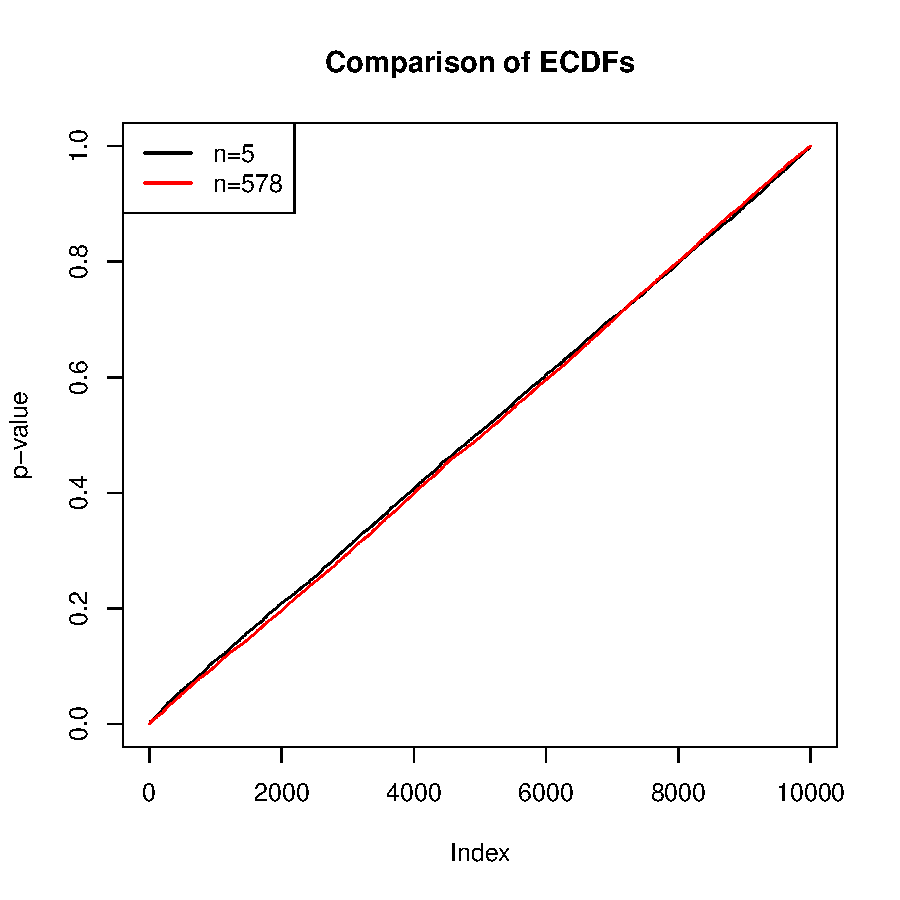
\includegraphics{multipletesting-001}
\end{Answer}

\begin{Exercise}
Say you work at level $\alpha=0.05$ on a null hypothesis $H_0$
that is true (but you do not know that). What is the probability
that you will reject $H_0$? If you test the hypothesis 2
times with independent datasets, what is the probability that you
will reject it none of the two times? If you test it $k$ times, what is 
the probability that you never reject it? If $k$ grows large, what
does this value tend to? So, if there is no limit on the number
of times a hypothesis is tested, what is the probability that it is
never rejected.
\end{Exercise}
\begin{Answer}
The probability of rejecting the null hypothesis when it is true
is by definition $\alpha$, \textit{i.e.} 0.05 in that case. If
you test it two times independently, the probability of accepting
it 2 times is $0.95 \times 0.95 = 0.902$. The multiplication comes
from the assumption of independence. If you test it $k$
times, the probability of accepting it $k$ times (never rejecting
it) is $0.95^k$. Because $0.95 < 1$, this value tends to 0 as $k$
increases. So, if there is no bound on $k$, the probability
of never rejecting the null hypothesis is 0.
\end{Answer}

\begin{Exercise}
What is most likely to be reported in the scientific literature:
rejection or acceptance of the null hypothesis? Regarding the
answer to the last question, what does that mean for published
knowledge?
\end{Exercise}
\begin{Answer}
Rejection is more likely to be published.
Accepted null hypothesis are almost never
reported as such. If a hypothesis is tested often enough, by the
same or different teams, the null hypothesis will be rejected
at some point, which will be published. Potentially any claim can
be reported in the literature.
\end{Answer}

\begin{Exercise}
Say that you test the same null hypothesis $H_0$ with two \textbf{non}
independent datasets (for example, one is the subset of the other)
and that the null hypothesis is true. What is the probability that
you will accept the null hypothesis both times?
\end{Exercise}
\begin{Answer}
We don't know. The only thing we can say is that the probability is
lower than 0.95. After the first test, the null hypothesis has been
accepted with probability 0.95. If it was accepted, the second test
has a probability $0 \leq p \leq 1$ of rejecting the test, so the
probability of accepting it both times is $(1-p) 0.95 \leq 0.95$.
The value of $p$ can really vary in the whole range between 0 and
1, so we cannot say more about it.
\end{Answer}


\begin{Exercise}
Generate 10000 p-values of a biased test. The test is as follows:
first do a $t$ test on two samples of size 5. If that is significant
at level $\alpha=0.05$, consider it significant and keep the p-value,
otherwise, add 5 more observations per sample and record the new
p-value, whether it is significant or not.
\end{Exercise}
\begin{Answer}
\begin{Schunk}
\begin{Sinput}
> p.bias <- rep(NA, 10000);
> for (i in 1:10000) {
+    x <- rnorm(5);
+    y <- rnorm(5);
+    p <- t.test(x,y)$p.value;
+    if (p < 0.05) {
+       p.bias[i] <- p;
+    }
+    else {
+       p.bias[i] <- t.test(c(x, rnorm(5)), c(y, rnorm(5)))$p.value;
+    }
+ }
> plot(sort(p.bias), type="S", main="Comparison of ECDFs",
+    ylab="p-value");
> lines(sort(p5), type="S", col=2);
> legend(x="topleft", legend=c("Biased test", "Single test"),
+    lwd=2, col=c(1,2));
\end{Sinput}
\end{Schunk}
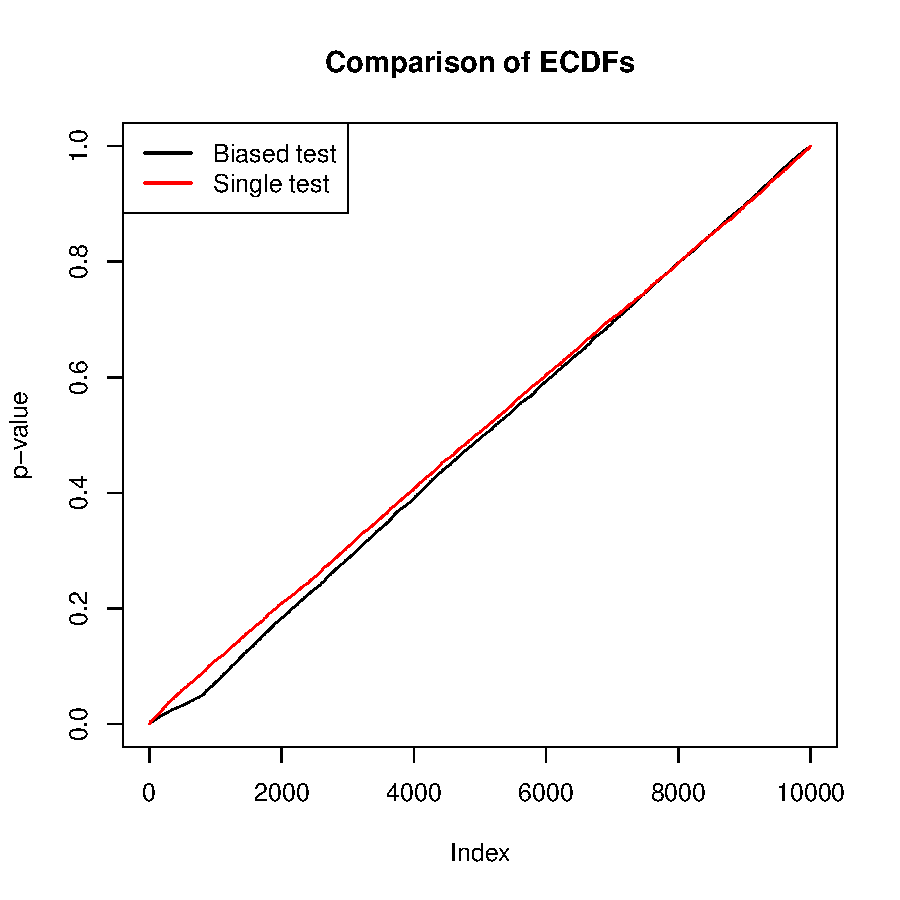
\includegraphics{multipletesting-002}
\end{Answer}

%% The Bonferroni correction %%
\section{The Bonferroni correction}

One of the ideas out there to deal with the problem is to somehow
take into account the number of times a hypothesis is tested.
As seen in exercise \ref{ugly}, this is not easy because every
scenario is possible.

A defining property of probabilities is that if $A$ and $B$ are
two events, $P(A \cup B)$, the probability that at least one
of these events occur is $P(A) + P(B) - P(A \cap B)$. This is
the basis for a correction method named after Carlo Emilio Bonferroni
(who did not actually invent the method).

\begin{Exercise}
\label{bonf}
Is it always true that $P(A \cup B) \leq P(A) + P(B)$?
\end{Exercise}
\begin{Answer}
Yes. Because probabilities are always positive or zero, taking out
the term $-P(A \cap B)$ on the right hand side of the equality gives
a bigger number. This is known as the Bonferroni inequality.
\end{Answer}

\begin{Exercise}
Suppose that you test a null hypothesis 2 times, and that this
hypothesis is true. Using the result of Exercise \ref{bonf}, give an
upper bound on the probability of rejecting the hypothesis at least
once.
\end{Exercise}
\begin{Answer}
If event $A$ is `the hypothesis is rejected in the first test' and
the event $B$ is `the hypothesis is rejected in the second test',
both have probability $\alpha$, and applying the Bonferroni inequality
says that the probability of rejecting the null hypothesis at least
once is $2 \alpha$.
\end{Answer}

\begin{Exercise}
Using Exercise \ref{bonf}, give an upper bound to
$P(A_1 \cup A_2 \cup ... \cup A_n)$.
\end{Exercise}
\begin{Answer}
\begin{eqnarray*}
  P(A_1 \cup A_2 \cup A_3 \cup ... \cup A_n)
    &=& P(A_1 \cup (A_2 \cup A_3 \cup ... \cup A_n)) \\
    &\leq& P(A_1) + P(A_2 \cup A_3 \cup ... \cup A_n) \\
    &\leq& P(A_1) + P(A_2 \cup A_3 \cup ... \cup A_n) \\
    &\leq& P(A_1) + P(A_2 \cup (A_3 \cup ... \cup A_n)) \\
    &\leq& P(A_1) + P(A_2) + P(A_3 \cup ... \cup A_n) \\
    &...& \\
    &\leq& P(A_1) + P(A_2) + P(A_3) + ... + P(A_n)
  \end{eqnarray*}
\end{Answer}

\begin{Exercise}
Based on this, give an upper bound on the probability of rejecting
a null hypothesis at least once out of $n$ tests, given that
this hypothesis is true. Say that you work at level $\alpha=0.05$
and that you test the same null hypothesis $n$ times. You will
reject the null hypothesis as a whole if it is rejected by at
least one of the individual tests. What has to be the level
$\tilde{\alpha}$ of each individual test so that you have a probability
less than $\alpha=0.05$ of rejecting the null hypothesis as a whole?
\end{Exercise}
\begin{Answer}
The upper bound is $n \times \times{\alpha}$.
If you set the level of individual tests to $\tilde{\alpha} = \alpha/n$,
the probability of rejecting the null hypothesis
as a whole is less than $n \times \alpha /n = \alpha$.
\end{Answer}

\begin{Exercise}
Assume you test $n$ different null hypotheses. Does the previous
rationale apply to this case as well? Should you correct the
p-values of the $n$ individual tests?
\end{Exercise}
\begin{Answer}
The rationale also holds, so you should correct for multiple testing.
\end{Answer}


\cleardoublepage
\shipoutAnswer
\end{document}
